\chapter{DOMAIN MODELING} \label{ch:procedure}

\section{Domain Modeling for Multi-Tenant E-Commerce System}

Domain modeling is the process of creating a conceptual representation of the business entities, their attributes, and relationships within a system, independent of technical implementation details. For the \textbf{Multi-Tenant E-Commerce System (M-TECS)}, domain modeling serves as the foundational blueprint that captures the core business concepts derived from the functional requirements.

\subsubsection*{Key Elements of the Domain Model}

\begin{itemize}
    \item \textbf{Core Entities:} The model identifies primary business classes including \texttt{Vendor}, \texttt{Customer}, \texttt{Product}, \texttt{Order}, \texttt{Payment}, \texttt{Delivery}, \texttt{Discount}, \texttt{Theme}, \texttt{Review}, and \texttt{Notification}—each representing a distinct business concept with relevant attributes.
    
    \item \textbf{Multi-Tenancy Support:} A critical aspect of the model is its explicit representation of data isolation through vendor-specific ownership. Classes such as \texttt{Product}, \texttt{Discount}, and \texttt{Theme} include \texttt{vendorId} attributes, ensuring that each tenant's data remains securely separated.
    
    \item \textbf{Relationships:} The model captures how entities interact, such as:
    \begin{itemize}
        \item A \texttt{Vendor} sells multiple \texttt{Products}
        \item A \texttt{Customer} places multiple \texttt{Orders}
        \item An \texttt{Order} contains multiple \texttt{OrderItems}
        \item A \texttt{Product} receives multiple \texttt{Reviews}
    \end{itemize}
    
    \item \textbf{Business Constraints:} Critical rules are documented, including:
    \begin{itemize}
        \item Customers can only review products they have purchased
        \item Product stock cannot be negative
        \item Discount end dates must follow start dates
    \end{itemize}
\end{itemize}

\subsubsection*{Significance}

The domain model serves multiple purposes:

\begin{itemize}
    \item \textbf{Communication:} Establishes a common vocabulary between technical and non-technical stakeholders.
    \item \textbf{Validation:} Ensures all functional requirements are represented conceptually.
    \item \textbf{Foundation:} Provides the basis for database design, detailed class diagrams, and implementation.
    \item \textbf{Reusability:} Creates a shared understanding that guides all subsequent development phases.
\end{itemize}

\section{Multi-Tenant E-Commerce System Domain Model Diagram}
\begin{figure}[H]
    \centering
    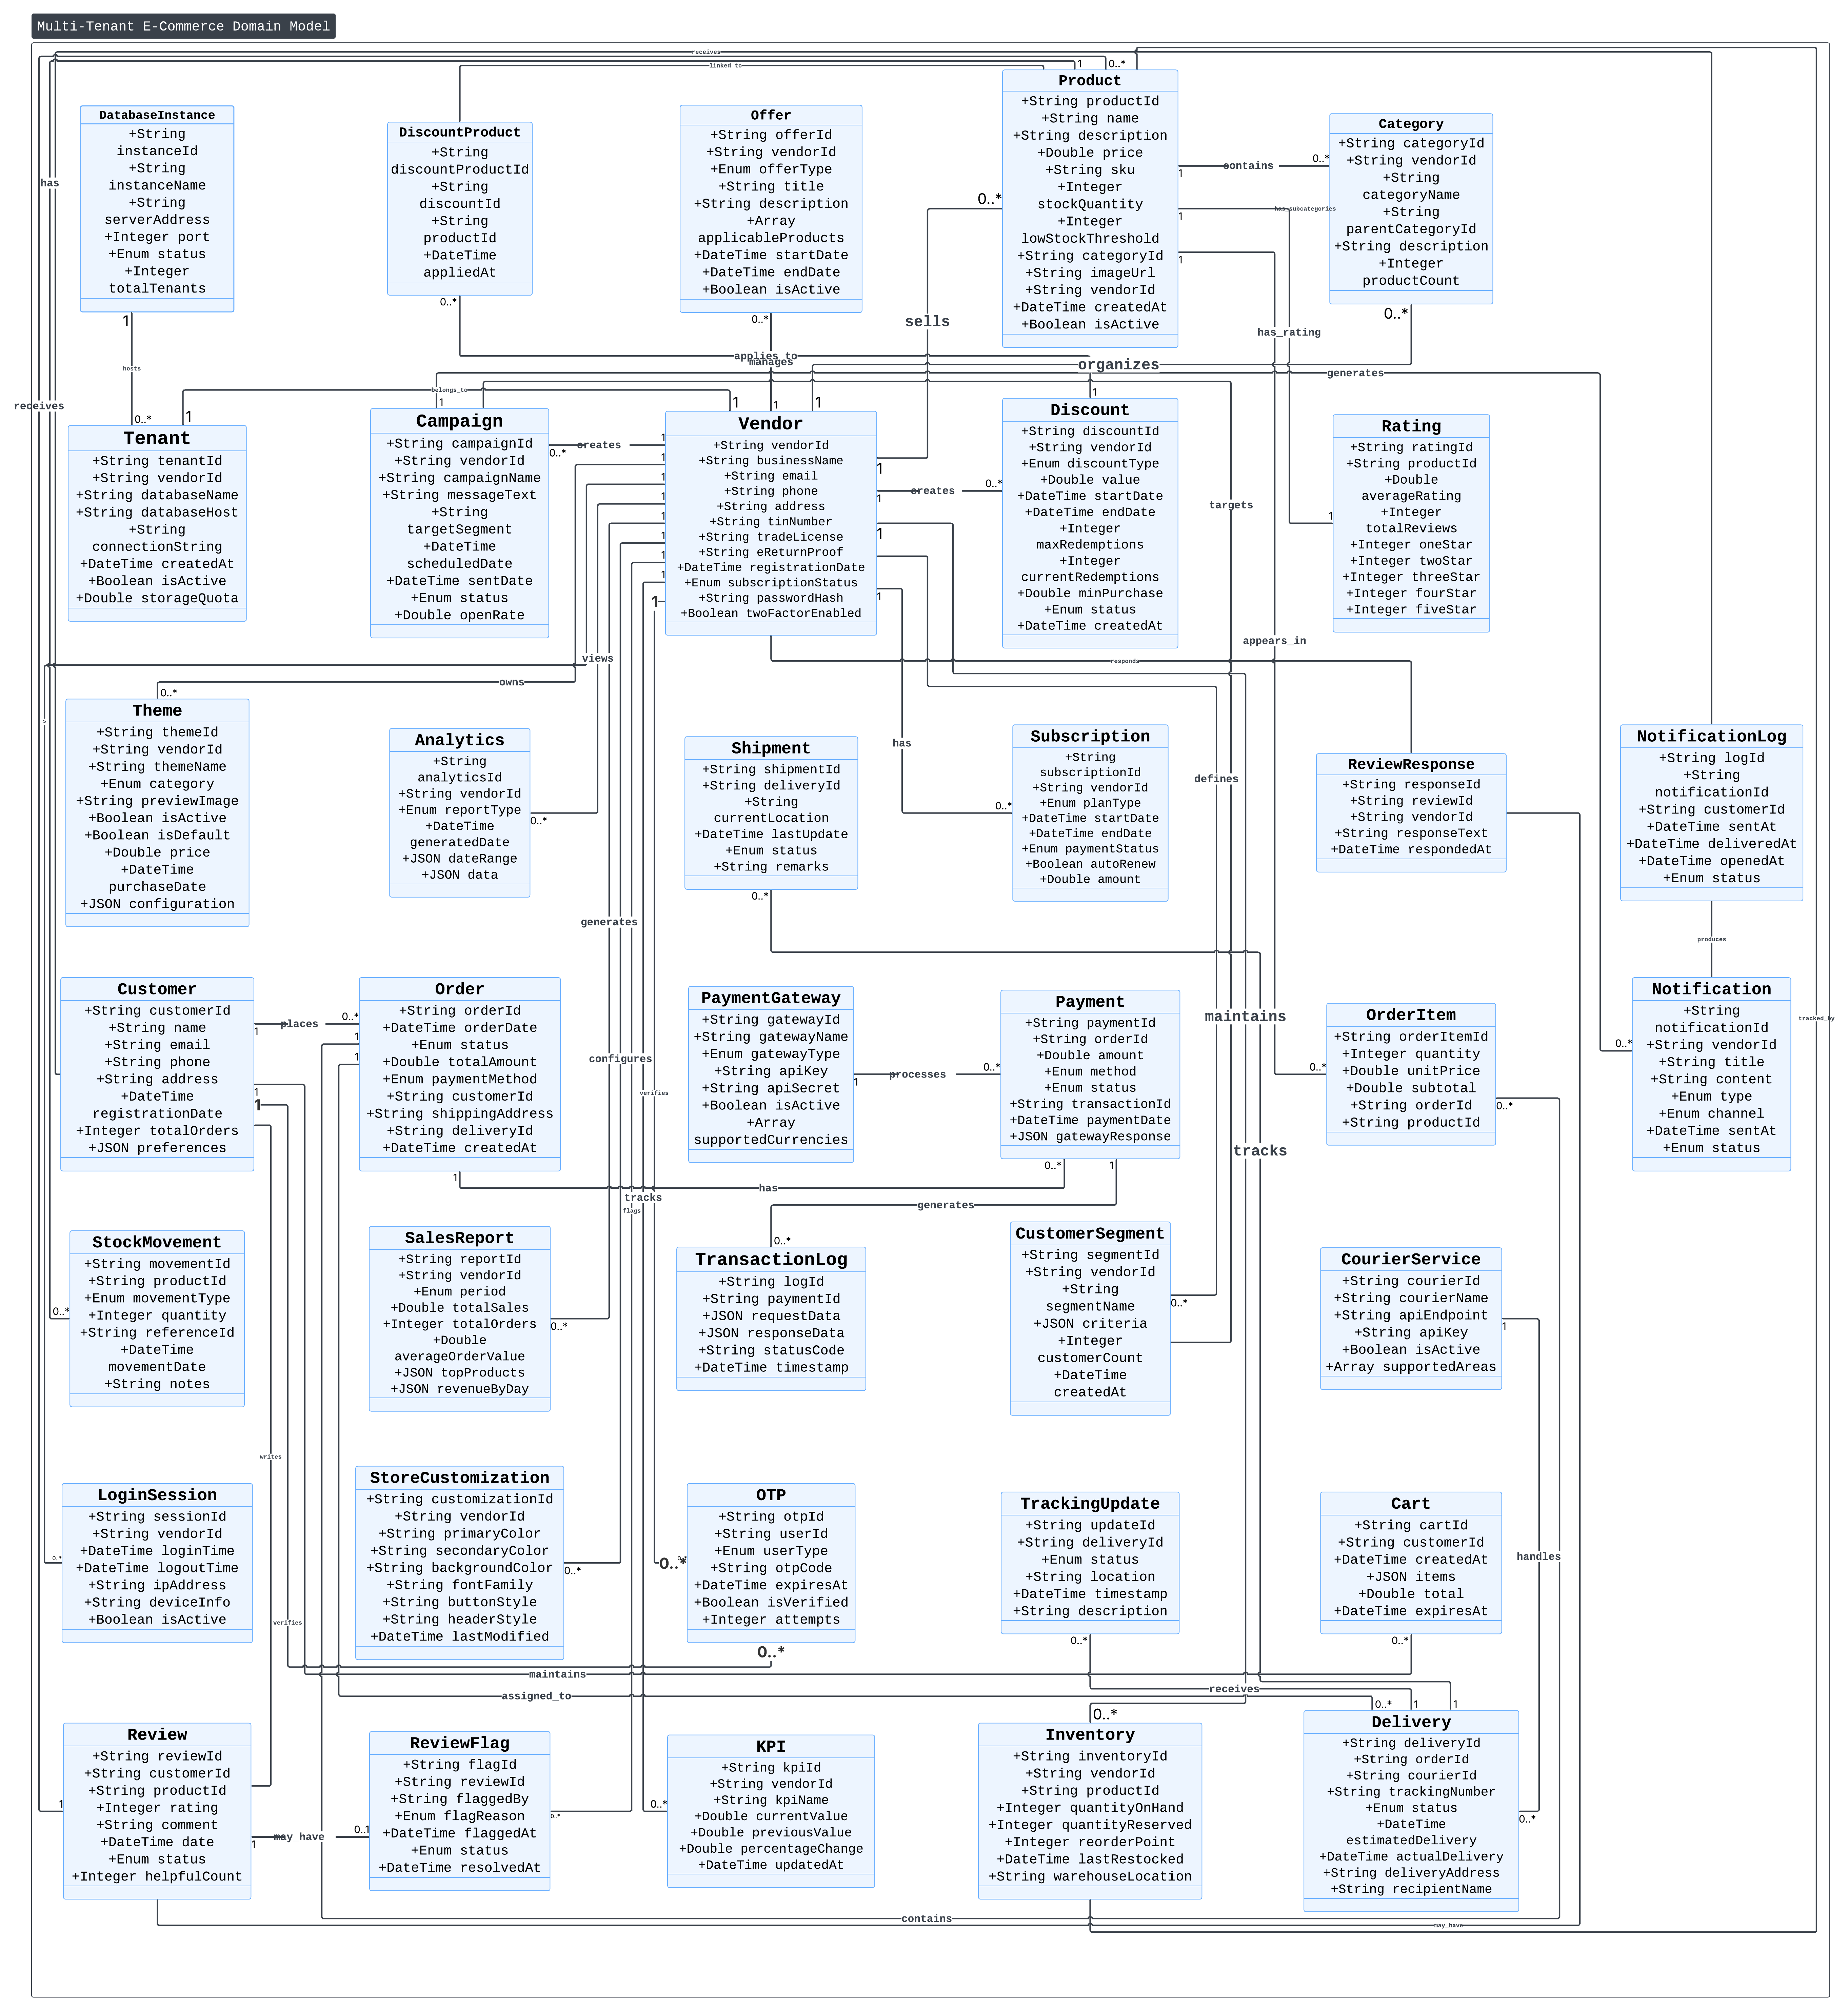
\includegraphics[width=1\linewidth]{figures/Domain Modeling 5A HQ.png}
    \caption{UML Domain Modeling of Multi-tenant E-commerce System}
    \label{fig:placeholder}
\end{figure}